\section{Simulation-Based Calibration Results}
\label{sec:sbc_results}

This section presents the results of SBC applied to validate the inference process for all models described in Chapter~\ref{methodology}.
The SBC procedure was performed independently for each model following the experimental design described in Section~\ref{sec:sbc_experimental_design}.

\subsection{Results for Club-Level Models}
\label{subsec:sbc_club}

The SBC validation was performed for all 14 club-level models: 4 Bradley-Terry variants (BT1--BT4) and 10 Poisson variants (P1--P10).
As shown in Table~\ref{tab:sbc_club_level}, no model exhibited more flagged parameters than expected by chance under the 95\% confidence bands.
Only four models (BT1, P3, P6, and P10) had a single parameter flagged, and in each case, the deviation was minimal: exactly 2 points outside the confidence envelope.
These results provide strong evidence that all club-level models are correctly implemented.

\begin{table}[htbp]
    \centering
    \begin{tabular}{lccccc}
        \toprule
        Model & Parameters & Expected & Flags & Points Out & Description \\
        \midrule
        BT1 & 20 & 1 & 1 & 2 & Single skill \\
        BT2 & 21 & 1 & 0 & 0 & BT1 + home effect \\
        BT3 & 21 & 1 & 0 & 0 & BT1 + ties \\
        BT4 & 22 & 1 & 0 & 0 & BT1 + home effect + ties \\
        \midrule
        P1  & 20 & 1 & 0 & 0 & Single skill \\
        P2  & 21 & 1 & 0 & 0 & P1 + home effect \\
        P3  & 40 & 2 & 1 & 2 & Attack/defence \\
        P4  & 41 & 2 & 0 & 0 & P3 + home effect \\
        P5  & 80 & 4 & 0 & 0 & Home/away split \\
        P6  & 21 & 1 & 1 & 2 & P1 + common effect \\
        P7  & 22 & 1 & 0 & 0 & P2 + common effect \\
        P8  & 41 & 2 & 0 & 0 & P3 + common effect \\
        P9  & 42 & 2 & 0 & 0 & P4 + common effect \\
        P10 & 81 & 4 & 1 & 2 & P5 + common effect \\
        \bottomrule
    \end{tabular}
    \caption{
        \textbf{SBC validation results for club-level models}.
        The ``Expected'' column shows the approximate number of parameters expected to be flagged by chance (5\% of total).
        All models show fewer flags than expected, confirming correct implementation.
    }
    \label{tab:sbc_club_level}
\end{table}

To illustrate what a flagged parameter looks like in practice, Figure~\ref{fig:sbc_club_examples} compares two skill parameters from model P6: $\alpha_1$ (flagged) and $\alpha_2$ (not flagged).
The visual difference is nearly imperceptible—both curves stay close to zero throughout, with $\alpha_1$ showing only a brief excursion beyond the confidence bands.
This comparison reinforces that the flagged cases represent statistical noise rather than systematic inference failures.

\begin{figure}[htbp]
    \centering
    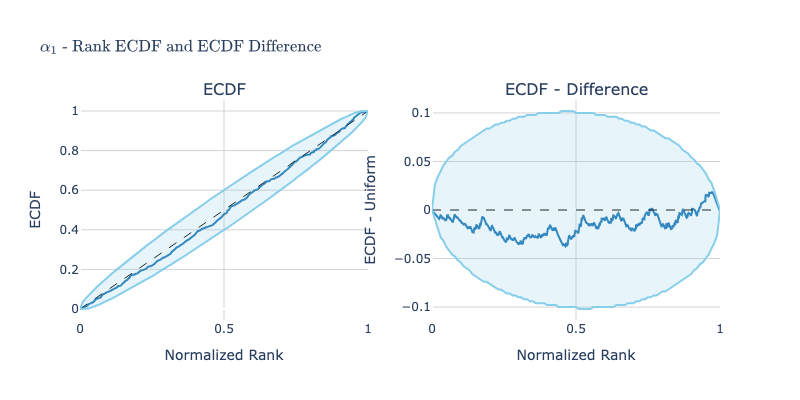
\includegraphics[width=\textwidth]{figures/alpha_1_ecdf_combined.png}
    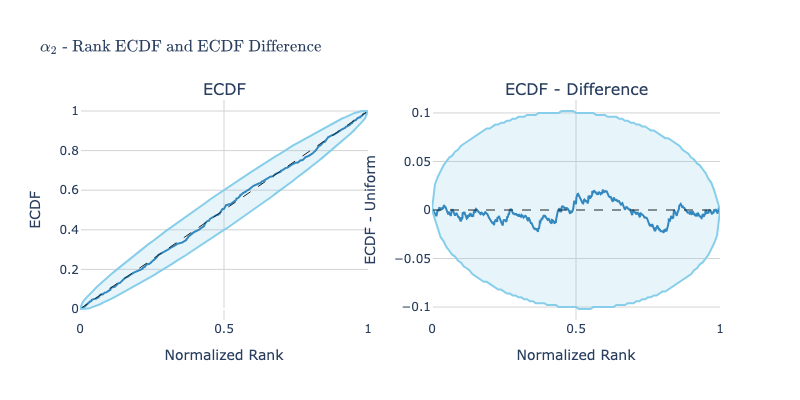
\includegraphics[width=\textwidth]{figures/alpha_2_ecdf_combined.png}
    \caption{
        \textbf{ECDF difference plots for model P6}.
        Top: the skill parameter $\alpha_1$, the only flagged parameter in this model, with exactly 2 points marginally outside the envelope.
        Bottom: the skill parameter $\alpha_2$, showing excellent calibration with all ranks within the 95\% confidence bands.
        Left panels show the empirical CDF of normalized ranks; right panels show the difference from the uniform distribution with 95\% confidence bands (shaded region).
        The contrast illustrates that even flagged parameters exhibit only minimal deviations.
    }
    \label{fig:sbc_club_examples}
\end{figure}

\subsection{Results for Player-Level Models}
\label{subsec:sbc_player}

The player-level models present a significant increase in dimensionality compared to their club-level counterparts.
For the SBC validation, synthetic datasets were generated with 732 unique players participating across the 380 matches of a season.
This includes a synthetic player capturing the effect of numerical disadvantage due to red cards.

Table~\ref{tab:sbc_player} summarizes the SBC results for the 8 player-level Poisson models.
Note that we evaluate fewer models at the player level compared to the club level.
Due to the high computational cost of player-level inference (hundreds to thousands of parameters per model), we restricted validation to a subset of models based on the club-level evaluation on real data (Section~\ref{sec:real_data}).
Bradley-Terry models were excluded as they performed below the Naive 2 baseline on BS, RPS and LS, indicating poor predictive ability.
Models P5 and P10 were also excluded due to severe over-fitting caused by their home/away split parametrization, performing worse than an uninformative baseline.
The remaining 8 Poisson models (P1--P4, P6--P9) were retained: models with home effect (P2, P4, P7, P9) for their strong predictive performance, and models without home effect (P1, P3, P6, P8) to validate the base model structures.

Despite the substantially higher number of parameters—ranging from 732 to 1,466 per model—the flagging rates remain low and consistent with chance.
For instance, model P9 has 1,466 parameters and would be expected to have approximately 73 flagged parameters (5\%) under the null hypothesis; only 10 were observed.
Similarly, model P3 with 1,464 parameters showed only 6 flags, far below the expected 73.

\begin{table}[htbp]
    \centering
    \begin{tabular}{lccccc}
        \toprule
        Model & Parameters & Expected & Flags & Points Out & Description \\
        \midrule
        P1  & 732   & 37 & 3  & 6  & Single skill \\
        P2  & 733   & 37 & 5  & 10 & P1 + home effect \\
        P3  & 1,464 & 73 & 6  & 14 & Attack/defence \\
        P4  & 1,465 & 73 & 8  & 16 & P3 + home effect \\
        P6  & 733   & 37 & 4  & 8  & P1 + common effect \\
        P7  & 734   & 37 & 4  & 8  & P2 + common effect \\
        P8  & 1,465 & 73 & 8  & 16 & P3 + common effect \\
        P9  & 1,466 & 73 & 10 & 20 & P4 + common effect \\
        \bottomrule
    \end{tabular}
    \caption{
        \textbf{SBC validation results for player-level models}.
        Despite the high dimensionality (up to 1,466 parameters), all models show far fewer flags than the expected 5\% rate.
    }
    \label{tab:sbc_player}
\end{table}

The flagged parameters correspond to individual player skills ($\alpha_i$ or $\beta_i$) distributed across different simulated players, with no systematic pattern.
Also, each flagged parameter had minimal deviations, as observed in club-level models.
These results confirm that the extension to high-dimensional player-level inference does not compromise calibration.
